\chapter{Introduction}
\label{chap:Introduction}

Lorem ipsum dolor sit amet, consectetur adipiscing elit. Pellentesque
rutrum vestibulum turpis porta facilisis. Integer volutpat suscipit
odio id adipiscing. Nulla convallis, odio quis tempus pharetra, ipsum
augue congue nibh, non auctor massa quam in urna. Proin tincidunt
vehicula lorem id fringilla. Integer pulvinar auctor rhoncus. Sed
aliquet metus in neque iaculis vulputate. Aliquam venenatis posuere
tempor. Maecenas gravida, lectus vitae facilisis viverra, ligula lacus
hendrerit odio, eu sagittis eros lectus quis tellus. Donec aliquam
lorem vitae urna varius tempus. Curabitur placerat egestas
hendrerit. Duis nisi magna, dignissim ac cursus id, luctus et
risus. In fermentum faucibus ultrices. Duis in libero ipsum. In quam
lacus, scelerisque et porttitor ac, molestie quis diam. Duis accumsan
pharetra ornare.

Morbi eget nunc ut justo viverra aliquam. Nulla sagittis viverra magna
at placerat. Pellentesque accumsan ullamcorper mi eget
laoreet. Pellentesque habitant morbi tristique senectus et netus et
malesuada fames ac turpis egestas. Quisque sit amet mi quis arcu
scelerisque gravida sit amet a odio. Integer a fringilla neque. Sed
blandit nisi convallis metus interdum sagittis. Suspendisse eu tellus
mi, rhoncus auctor dui. Pellentesque elementum turpis vitae lectus
luctus bibendum.



\section{A Section}
\label{sec:test}

Here is a section. 

\subsection{Subsection}
\label{subsec:s1}

Here is a subsection. 

Here \cite{2476800320070101} is a citation. This makes the reference
in bibliography.bib appear in the bibliography section. 

Here is a reference to another section: page \pageref{sec:another}.

Here is a figure that contains an image.

\begin{figure}[h!]
\centering
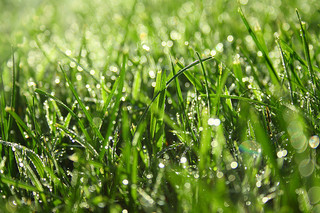
\includegraphics[scale=0.5]{figures/grass}
\caption{grass}
\label{fig:grass}
\end{figure}


And here is some code:
\begin{figure}[H]
\begin{singlespace}
\begin{lstlisting}[language=c]
    #include <stdio.h> 

    int main (int argc, char **argv) {
	    printf("Hello, World!\n");
        return 0;
    }
\end{lstlisting}
\end{singlespace}
\caption{Hello world}
\label{fig:hellocode}
\end{figure}

